
\chapter{Materials and Methods}

	This chapter details the research design and execution, providing sufficient information for others to verify or replicate the study, ensuring credibility and scientific rigor.
    
\section{Content Elements}
\subsection{Research Concept and Principles}
Explain the theoretical basis, such as physical principles or mathematical models.
\subsection{Experimental Design}

\begin{itemize}
    \item Describe hardware, software, material sources, sample preparation, and measurement procedures.
   \item Data Analysis: Outline data processing and analytical methods, such as statistical tools or algorithms.
   \item Rationale and Novelty: Justify the choice of methods and highlight their innovations.
   \item Visual Aids: Use schematic diagrams, flowcharts, or tables to clarify methods.

\end{itemize}


\section{Writing Tips}
\begin{itemize}
    \item Provide specific, reproducible details, avoiding vague descriptions.
    \item If methods build on prior work, clearly state improvements and cite sources.
    \item For complex methods, use subsections to enhance clarity and organization.
    \item For theoretical or qualitative studies, describe frameworks, data sources, or analytical approaches in detail.

\end{itemize}


\section{Inserting the figures}
\subsection{Insert Directly}

	Figure \ref{React} plots the surface iodine coverage $\theta$ as a function of $I_2$ exposure obtained from the STM images, and shows.... 
    
To prevent the List of Figures from displaying the entire caption, only write a short label in [~~] and write the full description of the figure in {~~~}, as shown below.

\begin{figure}[h]
\centering

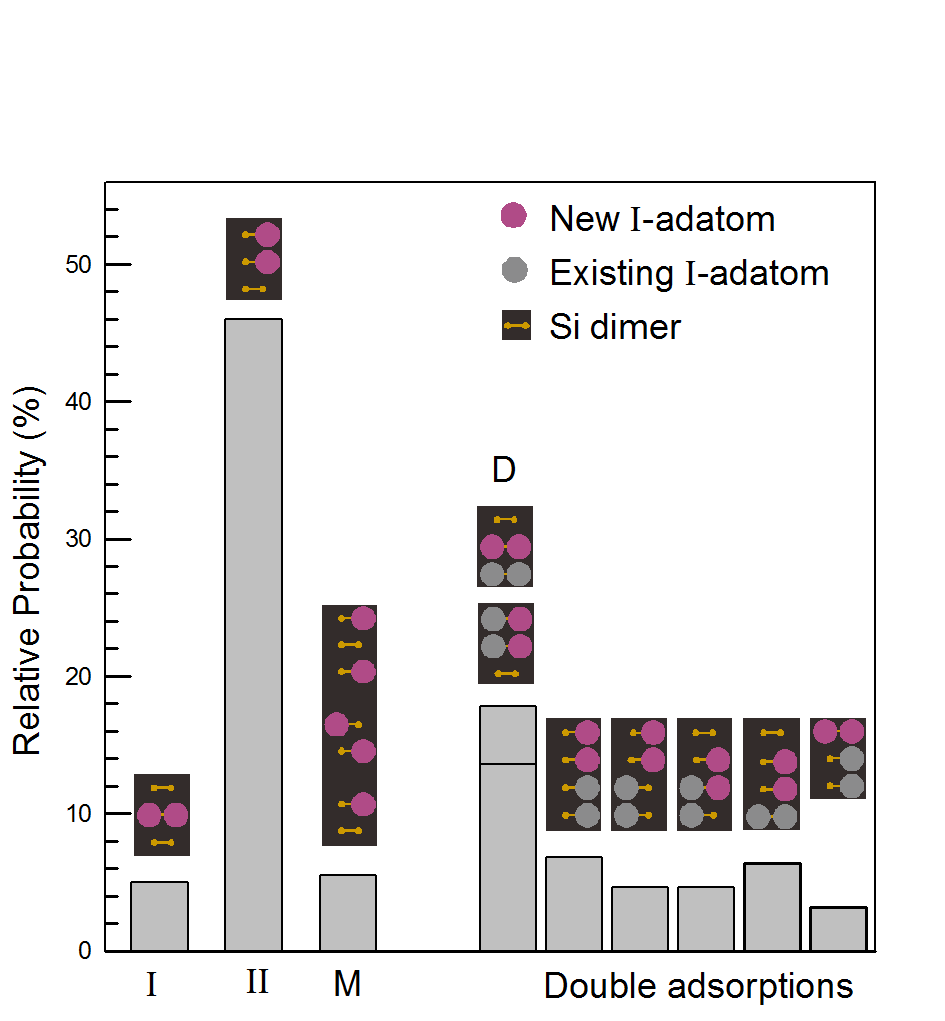
\includegraphics[width=.6\textwidth]{figures/ReactProbability.png}

\caption[Relative probabilities for various new adsorption configurations]{Relative probabilities for various new adsorption configurations as the iodine coverage on Si(100) increases from 0.10 to 0.14 ML. Type-I, type-II and type-M are new adsorption sites fully surrounded by dangling bonds. In double adsorptions, a new adsorption takes place next to an existing type-I or type-II adsorption site as the schematic models display.}
\label{React}

\end{figure}


This approach can also be used to insert tables, as shown below in Table \ref{tab:my_label1} Example of table here.


\begin{table}
    \centering
    %\begin{tabular}{ |p{2cm}||p{1.5cm}|p{1.5cm}|  }
    \begin{tabular}{ |c|c|c| } 
        \hline
        Structure  & 1 & 2\\
         \hline
         E& 2.0 & 3.8\\
          \hline
         H &  6.5 & 8.4 \\
    \hline
\end{tabular}
    \caption [Short version for LoF: Atomic arrangements and interaction energies]{Atomic arrangements and interaction energies for mixed adsorbates A and B in a $4\times4$ unit cell on Si(100). The energy for ($2\times1-p$), E8,AB, is the mean of the two energies for A- and B-terminated ($2\times1$) structure, respectively. }
    \label{tab:my_label1}
\end{table}


